\newif\ifglobal

%%%%%%%%%%%%%%%%%%%%%%%
%%% Compile to view %%%
%%%%%%%%%%%%%%%%%%%%%%%

%%%%%%%%%%%%%%%%%%%%%%%%%%%%%%%%%%%%%%%%%%%%%%%%%%%
%%% Readme:                                     %%%
%%% https://www.overleaf.com/read/bwdjvfjksvjy/ %%%
%%%%%%%%%%%%%%%%%%%%%%%%%%%%%%%%%%%%%%%%%%%%%%%%%%%

% >>> M?: marks a module setting number or important notice

% >>> M4: Set {./relative-path} to external files for this module <<<
\def \modulefiles {./62-TMPSEN}
% To add an external file, use:
% (Replace '---' with actual filename)
% '\input{\modulefiles/tables/---.tex}' for tables
% '\includegraphics{\modulefiles/figures/---}' for figures
% '\subfile{\modulefiles/---}' for register files

% >>> M1: This module is in global project? <<<
% 'YES' - uncomment; 'NO' - comment out
\globaltrue

\ifglobal
    \documentclass[main\_\_CN.tex]{subfiles}

\else
    % Font "FandolSong-Regular" used by ctex does not have GSUB table.
    % It causes warnings that do not affect compilation and can be ignored.
    \PassOptionsToPackage{quiet}{fontspec}

    \documentclass[openany, 10pt]{book}

    % >>> M2: In ./chip-spec-settings/preamble-trm-module, also find
    %         settings for visibility of todo notes, watermark <<<
    \usepackage{preamble-trm-module}


    % Enable Chinese typesetting
    \usepackage{ctex}

    % >>> M3: Temporary labels in Chinese
    %         you can add your own labels there <<<
    \myexternaldocument{temp-labels-cn}

\fi %\ifglobal


\setcounter{secnumdepth}{4}




% >>> M5: If this module needs any updates in
% './chip-spec-settings/preamble-trm-module.sty'
% (include additional package, etc.), contact your module PM
% or create the file './chip-spec-settings/changelog.tex' make the
% necessary updates yourself and document them in this file <<<

\raggedright


\begin{document}


% Sets language into which pre-defined bits of text are translated
\selectlanguage{chinese}

% Do not delete this block
\ifglobal
% Add the following front matter if
% this module is outside of global project
\else
    \InputIfFileExists{readme}{}{}
    {\let\clearpage\relax \listoftodos}
    {\let\clearpage\relax \listofdonetodos}
    \tableofcontents
    %\listoftables
    %\listoffigures
\fi


%%%%%%%%%%%%%%%%%%%%%%%%%
%%% TRM Module Begins %%%
%%%%%%%%%%%%%%%%%%%%%%%%%

\hypertarget{tmpsen}{}
\chapter{温度传感器 (TSENS)}
\label{mod:tmpsen}


\section{介绍}

\chipname{} 配备了一个温度传感器，用于实时测量芯片内部温度。温度传感器能将输出电压转换成数字值，并具有补偿温度偏移的功能。

\section{特性}

温度传感器的主要特性包括：
\begin{itemize}
    \item 支持软件触发测量温度，且一旦触发后，传感器可持续测量温度，软件可实时读取数据
    \item 支持硬件触发自动监测温度，支持两种自动监测唤醒模式
    \item 支持根据使用环境配置温度偏移，提高测试精度
    \item 温度测量范围可配置
\item 支持多个事件任务矩阵 (ETM) 相关的事件和任务
\end{itemize}

\section{结构概览}

温度传感器的内部结构如图 \ref{fig:tsens_struct} 所示。

\begin{figure}[H]
    \centering
    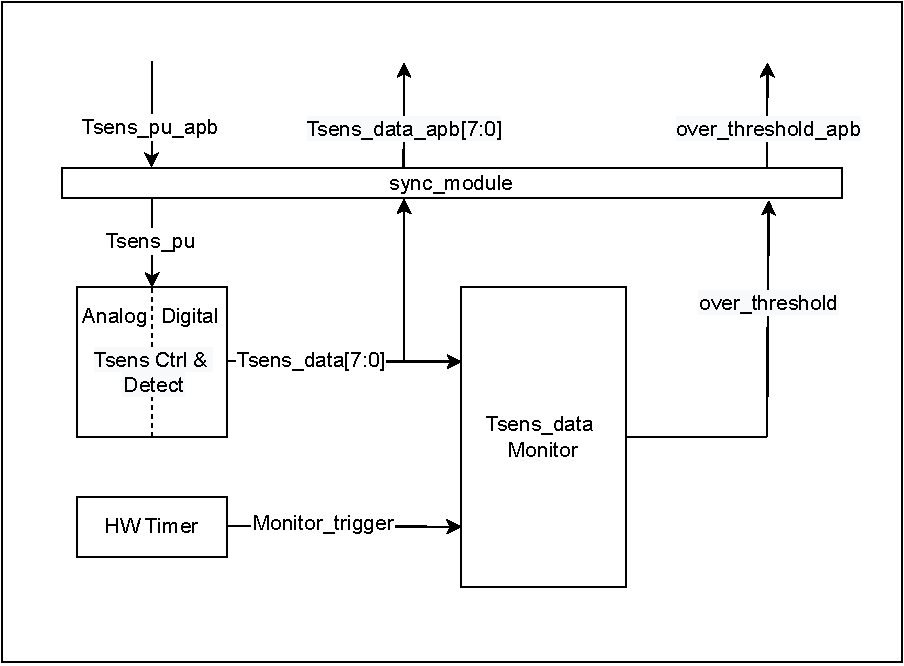
\includegraphics[width=0.8\textwidth]{62-TMPSEN/figures/tsens_struct_20221209}
    \caption{温度传感器结构框图}
    \label{fig:tsens_struct}
\end{figure}

根据图 \ref{fig:tsens_struct}，温度传感器模块主要包括以下功能模块：

\begin{itemize}
\item Tsens Ctrl \& Detect：温度传感器
    \item HW Timer（硬件定时器）：用于触发温度监测
    \item Tsens\_data 监测器：用于监测温度是否超出阈值
    \item sync\_module：APB 时钟域与温度传感器时钟域间的同步模块
\end{itemize}

\section{功能描述}

\subsection{温度传感器上电}
通过设置 \hyperref[fielddesc:TSENSPOWERUP]{TSENS\_POWER\_UP} 给温度传感器上电。

\subsection{时钟管理}
温度传感器只有一个时钟源：LP\_PERI\_CLK，并且没有时钟分频寄存器。

\subsection{自动监测唤醒模式}

温度传感器的自动温度监测功能有两种唤醒模式：绝对值模式和变化量模式，通过寄存器 \hyperref[fielddesc:TSENSWAKEUPMODE]{TSENS\_WAKEUP\_MODE} 进行选择。

   \begin{itemize}
       \item 绝对值模式：
           \begin{itemize}
                \item 用于监测当前温度的绝对值。配置 \hyperref[fielddesc:TSENSWAKEUPTHLOW]{TSENS\_WAKEUP\_TH\_LOW} 和 \hyperref[fielddesc:TSENSWAKEUPTHHIGH]{TSENS\_WAKEUP\_TH\_HIGH} 来决定温度阈值，温度超过高阈值或小于低阈值时将触发唤醒。
           \end{itemize}
       \item 变化量模式：
            \begin{itemize}
                \item 用于监测温度的变化量。若连续两次采样的温度值增量超过 \hyperref[fielddesc:TSENSWAKEUPTHHIGH]{TSENS\_WAKEUP\_TH\_HIGH} 的配置值或减少量超过 \hyperref[fielddesc:TSENSWAKEUPTHLOW]{TSENS\_WAKEUP\_TH\_LOW} 的配置值，将触发唤醒。例如当 \hyperref[fielddesc:TSENSWAKEUPTHLOW]{TSENS\_WAKEUP\_TH\_LOW} 的值为 8 时，若连续两次温度采样分别为 28 和 19，即温度减少量为 9，将触发唤醒。
            \end{itemize}
    \end{itemize}

\subsection{温度测量范围与温度偏移}

为了提高测试精度，温度传感器的测量范围被设计为 5 个范围，如表 \ref{tab:tsensor-dac} 所示。每个测量范围都有一定的测温误差。用户无需关注测温误差，只需选择相应的温度偏移，即可获得校准后的数据。

\begin{longtable}[c]{|l|r|}
    \caption{温度测量范围与温度偏移}
    \label{tab:tsensor-dac}
    \\\hline
    \rowcolor{lightgray}
    \textbf{测量范围 (°C)}  & \textbf{温度偏移} \\\hline
    50 \verb+~+ 125 & –2 \\\hline
    20 \verb+~+ 100 &  –1 \\\hline
    –10 \verb+~+ 80 &  0 \\\hline
    –30 \verb+~+ 50 &  1 \\\hline
    –40 \verb+~+ 20 &  2 \\\hline
\end{longtable}

\subsection{数据转换}

温度传感器的输出值 \(VALUE\) 存储在寄存器 \hyperref[fielddesc:TSENSOUT]{TSENS\_OUT} 中。用户可使用以下公式将输出值 \(VALUE\) 转换成实际的温度值 \(T\) (°C)。转换公式如下：

\[
        T = 0.4386 × VALUE – 27.88 × offset – 20.52
\]

其中，\(offset\) 即表 \ref{tab:tsensor-dac} 所示温度偏移。

%%%%%%%%%%%%%%%%%%%%%%%%%%%%%%%%%
%%% Event Task Matrix Feature %%%
%%%%%%%%%%%%%%%%%%%%%%%%%%%%%%%%%

\section{事件任务矩阵功能}
\label{sec:sensor-etm-func}

在 \chipname{} 中，温度传感器支持 ETM 功能，即可以通过任意外设的 ETM 事件触发 温度传感器的 ETM 任务，或者通过温度传感器的 ETM 事件触发任意外设的 ETM 任务。关于 ETM 更多详细信息，请参考章节 \ref{mod:evntaskmatrix} \nameref{mod:evntaskmatrix}。这里仅介绍与温度传感器相关的 ETM 任务和 ETM 事件。

温度传感器可接收的 ETM 任务有：

\begin{itemize}
    \item TMPSNSR\_TASK\_START\_SAMPLE：该任务被触发时，温度传感器开始采样。
    \item TMPSNSR\_TASK\_STOP\_SAMPLE：该任务被触发时，温度传感器停止采样。
\end{itemize}

温度传感器可产生的 ETM 事件有：

\begin{itemize}
    \item TMPSNSR\_EVT\_OVER\_LIMIT：温度传感器发现温度超过阈值时生成。
\end{itemize}

在具体应用中，温度传感器的 ETM 事件可以用来触发温度传感器的 ETM 任务，例如，TMPSNSR\_EVT\_OVER\_LIMIT 事件可以触发 TMPSNSR\_TASK\_STOP\_SAMPLE 任务。

%%%%%%%%%%%%%%%%%%%%%
%%% Interrupts %%%
%%%%%%%%%%%%%%%%%%%%%

\section{中断}

\chipname{} 的温度传感器可以生成以下中断信号并发送给\hyperref[mod:intmtrx]{中断矩阵}。

    \begin{itemize}
        \item LP\_TSENS\_INTR
    \end{itemize}

这个中断信号由以下内部中断源生成：
    \begin{itemize}
        \item TSENS\_COCPU\_TSENS\_WAKE\_INT\label{int:TSENSINT}：当温度样本值超过阈值时触发。
    \end{itemize}

\begin{tiplisting}
中断、中断源、中断信号等术语的解释以及它们之间的联系请参考章节 \ref{mod:intmtrx} \textit{\nameref{mod:intmtrx}} > \ref{sec:intmtx-int-terminology} \textit{\nameref{sec:intmtx-int-terminology}}。
\end{tiplisting}

每个中断源都有一组通用的配置寄存器，详见章节 \hyperref[interrupt-config-registers]{\textit{中断配置寄存器}}。具体寄存器名称请查看 \ref{sec:tmpsen-reg-summ} \textit{\nameref{sec:tmpsen-reg-summ}}。

\section{配置流程}

温度传感器可由软件启动，具体配置如下：
    \begin{enumerate}
        \item 置位 \hyperref[fielddesc:TSENSPOWERUP]{TSENS\_POWER\_UP} 使温度传感器上电；
        \item 置位 \hyperref[fielddesc:LPPERICKENLPTSENS]{LPPERI\_CK\_EN\_LP\_TSENS} 使能温度传感器时钟；
        \item 等待 \hyperref[fielddesc:TSENSXPDWAIT]{TSENS\_XPD\_WAIT} 个时钟周期后，温度传感器的复位释放，开始测量环境温度；
        \item 等待 100 $\mu$s 后（输出值会随着测量时间的增加而逐渐逼近真实的温度值），直接从 \hyperref[fielddesc:TSENSOUT]{TSENS\_OUT} 中读取温度值。
    \end{enumerate}

如要使用硬件自动温度监测功能，则可在给温度传感器上电之前增加如下步骤：
    \begin{enumerate}
        \item 配置 \hyperref[fielddesc:TSENSSAMPLERATE]{TSENS\_SAMPLE\_RATE} 设置采样率；
        \item 配置 \hyperref[fielddesc:TSENSWAKEUPMODE]{TSENS\_WAKEUP\_MODE} 选择温度监测唤醒模式；
        \item 配置 \hyperref[fielddesc:TSENSWAKEUPTHHIGH]{TSENS\_WAKEUP\_TH\_HIGH/LOW} 设置温度高低阈值；
        \item 置位 \hyperref[fielddesc:TSENSWAKEUPEN]{TSENS\_WAKEUP\_EN} 启用温度监测；
        \item 置位 \hyperref[fielddesc:TSENSSAMPLEEN]{TSENS\_SAMPLE\_EN} 自动触发持续温度监测。
    \end{enumerate}

自动温度监测工作模式下，温度传感器的输出值不会存储，但用户可以随时读取寄存器 \hyperref[fielddesc:TSENSOUT]{TSENS\_OUT} 获取当前输出值。


% >>> If your module has no registers, delete sample text
%       for Sections Register Summary and Registers below <<<

%%%%%%%%%%%%%%%%%%%%%%%%
%%% Register Summary %%%
%%%%%%%%%%%%%%%%%%%%%%%%

% >>> Update the sample text below and insert
%     the info on register summary into the subfile <<<

\newpage
\hypertarget{tmpsen-reg-summ}{}
\section{寄存器列表}
\label{sec:tmpsen-reg-summ}

本小节的所有地址均为相对于温度传感器基地址的地址偏移量（相对地址），具体基地址请见章节 \ref{mod:sysmem} \textit{\nameref{mod:sysmem}} 中的表 \ref{tab:sysmem-base-address}。

请查看章节 \hyperref[glossary-access-types]{\textit{寄存器的访问类型}}，了解“访问”列缩写的含义。

\subfile{\modulefiles/62-TMPSEN-reg-summ__CN}


%%%%%%%%%%%%%%%%%
%%% Registers %%%
%%%%%%%%%%%%%%%%%

% >>> Update the sample text below and insert
%      the info on registers into the subfile <<<

\newpage
\section{寄存器}

本小节的所有地址均为相对于温度传感器基地址的地址偏移量（相对地址），具体基地址请见章节 \ref{mod:sysmem} \textit{\nameref{mod:sysmem}} 中的表 \ref{tab:sysmem-base-address}。

关于保留 (reserved) 域的处理，请查看章节 \hyperref[programming-reserved-field]{如何配置寄存器的保留域}。

\subfile{\modulefiles/62-TMPSEN-reg__CN}


\end{document}
